\section{Case or Rule}
\subsection{case-based and rule-based 的原理}
\begin{frame}{case-based and rule-based 的原理}
	% \begin{itemize}[<+-| alert@+>] % 当然,除了alert,手动在里面插 \pause 也行
	%     \item 大家可能会\LaTeX{},不会的也会GPT,好多学校都有自己的Beamer主题
	%     \item 中文支持请选择 Xe\LaTeX{} 编译选项
	%     \item 原 THU Beamer 的项目地址位于 \url{https://github.com/tuna/THU-Beamer-Theme}
	%     \item 本项目地址位于 \url{https://github.com/Lanthanum1/CCNU-Beamer},如果有bug或者feature request可以去提issue
	% \end{itemize}
	\begin{columns}
		\begin{column}{0.2\textwidth}\onslide<2->{
				case-based 依赖训练时的语料库,如果语料库中没有需要推理的这个问题,则准确度会大幅下降。
			}
		\end{column}
		% \pause
		\begin{column}{0.6\textwidth} \onslide<1->{
				\begin{figure}[t]
					\centering        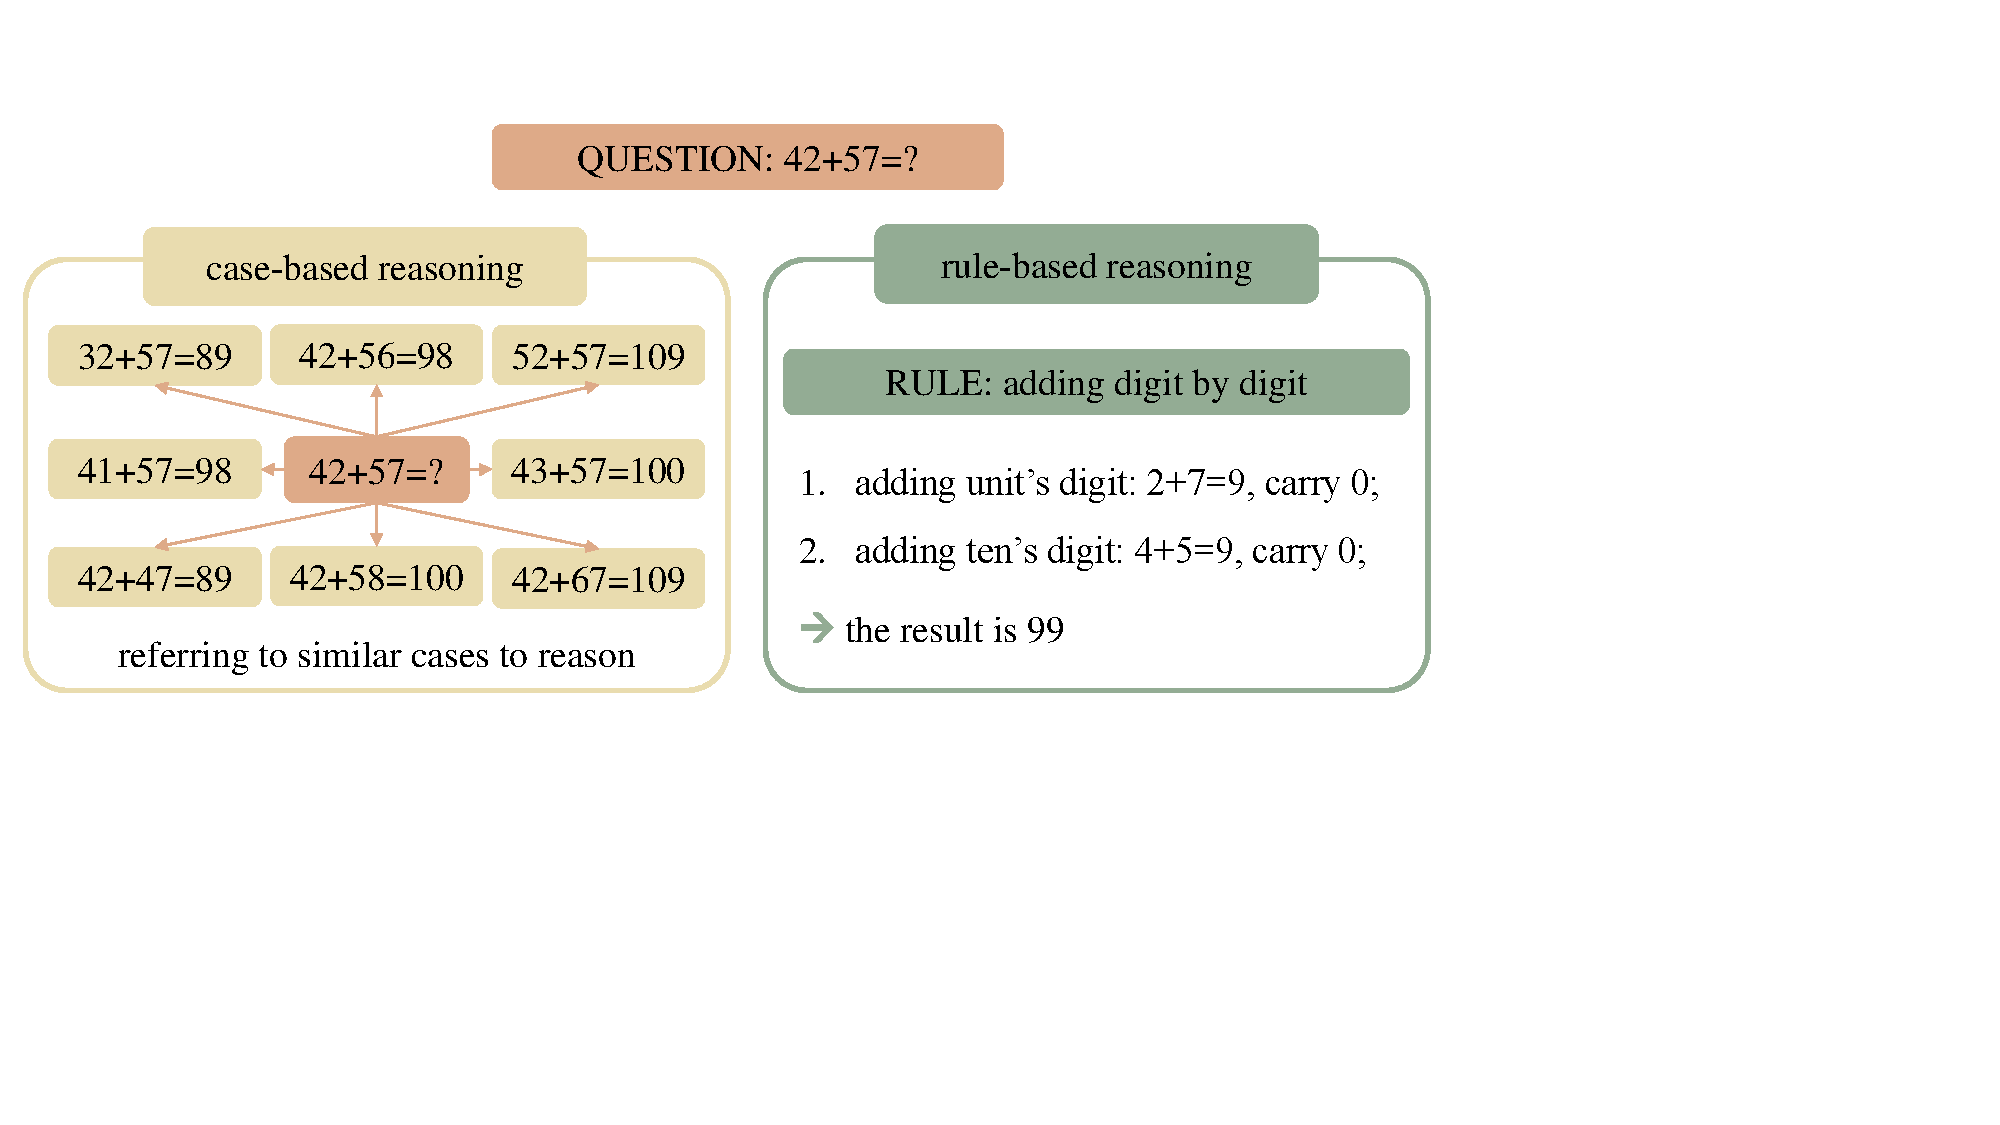
\includegraphics[width=\textwidth]{pic/case-or-rule.pdf}
					\caption{Illustrations of case-based and rule-based reasoning.}
					\label{case-or-rule}
				\end{figure}
			}
		\end{column}
		% \pause
		\begin{column}{0.2\textwidth}\onslide<3->{
				rule-based 依赖数学规则,即使语料库中没有这个问题,也可以根据从语料库中学习到的数学规则推理出正确的答案。}
		\end{column}
	\end{columns}
\end{frame}

\subsection{Leave-Square-Out method}
\begin{frame}{Leave-Square-Out method} \small
	% \begin{exampleblock}{什么是Leave-Square-Out method?}
	Leave-Square-Out method (留方法,LSO) 是作者提出的一种交叉验证(cross-validation)方法,用于评估机器学习模型的性能。它是留一法(Leave-One-Out)的扩展。与留一法相比,Leave-Square-Out 方法不是每次只留一个样本进行测试,而是每次留出 $k^2$ 个样本进行测试,其中 $k$ 是一个正整数。当数据集规模较大时,这种方法可以更好地评估模型的泛化能力。
	\pause
	% \end{exampleblock}
	\begin{figure}[t]
		\centering
		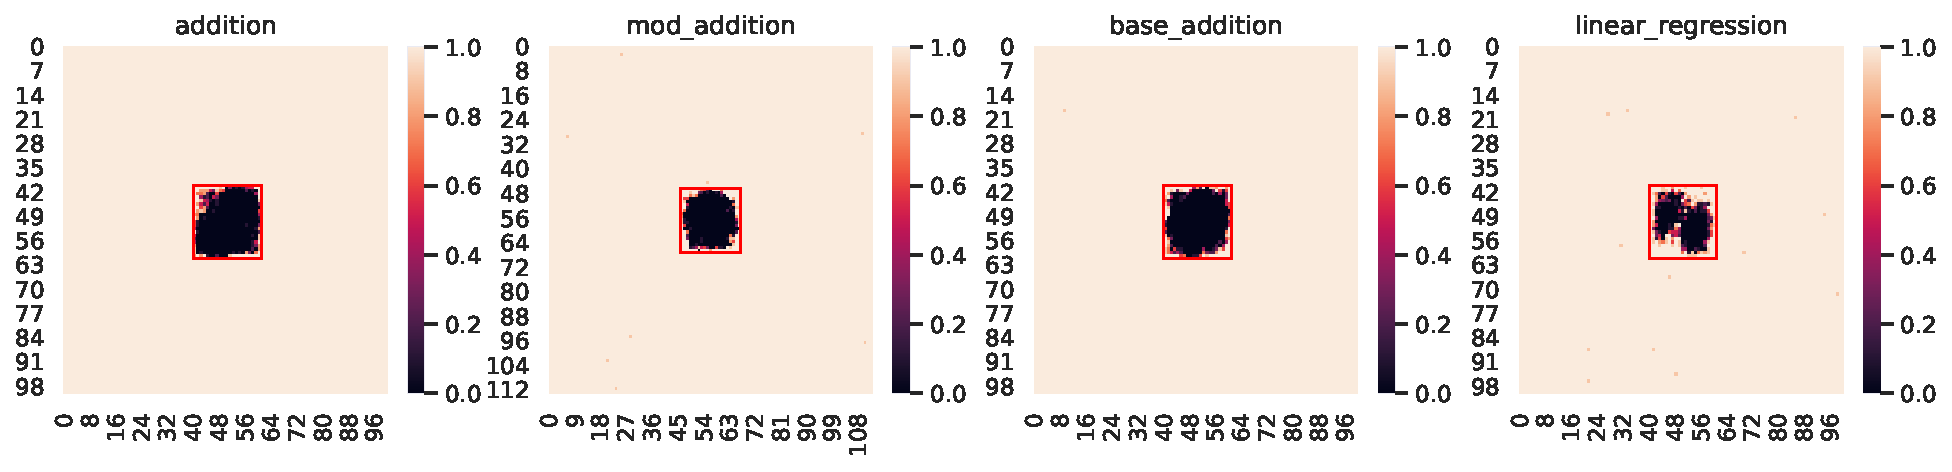
\includegraphics[height=0.3\textheight]{pic/1holes_w_rec_red_compressed.pdf}
		% \vspace{-10pt}
		\caption{Accuracy of Leave-Square-Out method}
		\label{fig:holes}
	\end{figure}
	\pause
	The appearance of holes in the figure indicates that the test samples away from the boundary of the training set are hard for the models to correctly infer.
\end{frame}

\subsection{rule-based setting}
\begin{frame}{rule-based setting}
	\begin{exampleblock}{rule based 的重要性}
		Rule-based reasoning is essential for models to achieve systematic and length generalization so that they can be applied to new, unseen scenarios without re-training.
	\end{exampleblock}
	\pause
	\begin{exampleblock}{rule based 应注意的事情}
		training set should always provide the necessities for the model to learn the underlying rule. For example, the training set should at least cover all the tokens used in the test set in order to develop a systematic rule that applies to the whole dataset.
	\end{exampleblock}

\end{frame}

\subsection{实验结论}
\begin{frame}{实验结论}
	\begin{itemize}
		\item test squares 的位置不会影响实验结果
		      \pause
		\item test squares 的大小会影响实验结果(the hole disappears when the test square shrinks to less than a small size)
		      \pause
		\item scratchpad cannot teach transformers to perform rule-based reasoning. (why? scratchpad fine-tuning fails to teach transformers the actually applied "rule" behind each step. This is like teaching children addition only by showing them examples, without telling them the rationales behind each step.)
		      \pause
		\item 模型和数据集的增大几乎不会影响实验结果,“holes”仍然存在
	\end{itemize}
\end{frame}
